\documentclass[11pt,a4paper]{article}
\usepackage[utf8]{inputenc}
\usepackage[T1]{fontenc}
\usepackage[spanish,es-noshorthands]{babel}
\usepackage[margin=2.5cm]{geometry}
\usepackage{parskip}
\usepackage{hyperref}
\usepackage{enumitem}
\usepackage{booktabs}
\usepackage{array}
\usepackage{xcolor}
\usepackage{graphicx}
\usepackage{longtable}
\usepackage{amsmath}
\usepackage{amssymb}

\definecolor{done}{RGB}{0,140,0}
\definecolor{partialcol}{RGB}{200,120,0}
\definecolor{pendingcol}{RGB}{180,0,0}
\definecolor{bugcol}{RGB}{140,0,140}

\setlength{\parindent}{0pt}
\setlength{\parskip}{6pt}

\hypersetup{colorlinks=true, linkcolor=black, urlcolor=blue}

\title{\textbf{Plan de migración a ROS para navegación}\\[6pt]
\large VLMaps + YOLOE + Habitat-Sim \,$\rightarrow$\, ROS para navegación y futura integración con HSR}
\author{Mario García Blasco}
\date{23 de abril de 2026 (revisión)}

\begin{document}

\maketitle
\section*{Chuleta operativa ROS/Gazebo}

Esta sección se mantiene como lista viva de comandos prácticos para lanzar el
\emph{stack} ROS sin depender de menús. La idea es poder ejecutar siempre lo
esencial a mano, primero desde el host para arrancar el contenedor y después
desde dentro de \texttt{tfg-ros} para compilar, lanzar Gazebo o inspeccionar
topics.

\paragraph{1. Arrancar el contenedor ROS desde el host.}

\begin{verbatim}
cd /home/mario/tfg/vlmap-semantic-object-search-tfg/docker
docker compose up -d tfg-ros
docker exec -it tfg-ros bash
\end{verbatim}

\paragraph{2. Compilar el workspace ROS dentro de \texttt{tfg-ros}.}

\begin{verbatim}
cd /ros_ws
catkin build
\end{verbatim}

\paragraph{3. Lanzar HSR oficial sólo en Gazebo.}

\begin{verbatim}
roslaunch vlmap_bringup hsr_gazebo_only.launch gui:=true use_rviz:=false
\end{verbatim}

\paragraph{4. Lanzar HSR oficial en Gazebo con RViz.}

\begin{verbatim}
roslaunch vlmap_bringup hsr_gazebo_only.launch gui:=true use_rviz:=true
\end{verbatim}

\paragraph{5. Lanzar HSR oficial en mundo simple y estático.}

\begin{verbatim}
roslaunch vlmap_bringup hsr_gazebo_simple.launch
\end{verbatim}

\paragraph{6. Lanzar HSR oficial en interior estático validado.}

\begin{verbatim}
roslaunch vlmap_bringup hsr_gazebo_indoor.launch
\end{verbatim}

Este preset usa \texttt{willowgarage.world} con una pose verificada dentro del
contenedor y un perfil de cabeza corregido para que la RGB-D vea un pasillo útil
en vez de techo/pared.

\paragraph{7. Lanzar stack completo con HSR oficial.}

\begin{verbatim}
roslaunch vlmap_bringup hsr_gazebo_move_base.launch \
  gui:=true use_rviz:=false use_rosbridge:=false
\end{verbatim}

\paragraph{8. Lanzar stack completo con HSR oficial y RViz.}

\begin{verbatim}
roslaunch vlmap_bringup hsr_gazebo_move_base.launch \
  gui:=true use_rviz:=true use_rosbridge:=false
\end{verbatim}

\paragraph{9. Lanzar HSR oficial en un mundo concreto.}

\begin{verbatim}
roslaunch vlmap_bringup hsr_gazebo_only.launch \
  world:=/usr/share/gazebo-11/worlds/willowgarage.world \
  gui:=true use_rviz:=true
\end{verbatim}

\paragraph{10. Teleoperar el HSR oficial por teclado.}

\begin{verbatim}
rosrun vlmap_bringup hsr_keyboard_teleop.py
\end{verbatim}

Este \texttt{teleop} publica en \texttt{/hsrb/command\_velocity}, que ahora
alimenta el controlador de base del HSR oficial en Gazebo; ya no depende del
robot \emph{proxy}.

\paragraph{11. Ver topics relevantes del HSR.}

\begin{verbatim}
rostopic list | egrep 'hsrb|move_base|vlmap|scan|image_rect|camera_info|rectified_points'
\end{verbatim}

\paragraph{12. Inspeccionar cámaras y sensores.}

\begin{verbatim}
rostopic hz /hsrb/base_scan
rostopic echo -n 1 /hsrb/head_rgbd_sensor/rgb/camera_info
rostopic echo -n 1 /hsrb/head_rgbd_sensor/depth_registered/camera_info
\end{verbatim}

\paragraph{13. Ver el árbol TF.}

\begin{verbatim}
rosrun tf view_frames
\end{verbatim}

\paragraph{14. Parar Gazebo, RViz y launches activos.}

\begin{verbatim}
pkill -f 'roslaunch vlmap_bringup'
pkill -f gzserver
pkill -f gzclient
pkill -f 'rosrun rviz rviz'
\end{verbatim}

\paragraph{15. Reiniciar limpio el contenedor ROS desde el host.}

\begin{verbatim}
cd /home/mario/tfg/vlmap-semantic-object-search-tfg/docker
docker compose up -d --force-recreate tfg-ros
\end{verbatim}

\paragraph{16. Panel RViz de depuración visual.}

\begin{verbatim}
roslaunch vlmap_bringup hsr_gazebo_only.launch gui:=true use_rviz:=true
\end{verbatim}

Con ese launch, en RViz conviene comprobar al menos:
\begin{itemize}
  \item \texttt{RobotModel}: el HSR aparece completo y no colapsa cabeza o
        brazo.
  \item \texttt{TF}: existen \texttt{map}, \texttt{odom},
        \texttt{base\_footprint}, \texttt{base\_link} y los frames de cámara.
  \item \texttt{LaserScan}: el topic \texttt{/hsrb/base\_scan} dibuja lecturas.
  \item \texttt{Image}: la RGB publica en
        \texttt{/hsrb/head\_rgbd\_sensor/rgb/image\_rect\_color}.
  \item \texttt{PointCloud2}: la nube de puntos llega desde
        \texttt{/hsrb/head\_rgbd\_sensor/depth\_registered/rectified\_points}.
\end{itemize}

\paragraph{15. Comandos de depuración RViz/TF/cámaras.}

\begin{verbatim}
rostopic echo -n 1 /tf
rostopic hz /hsrb/head_rgbd_sensor/rgb/image_rect_color
rostopic hz /hsrb/head_rgbd_sensor/depth_registered/rectified_points
rosrun rqt_image_view rqt_image_view
\end{verbatim}

\paragraph{16. Mundo Gazebo mínimo para probar la GUI.}

\begin{verbatim}
roslaunch gazebo_ros empty_world.launch gui:=true
\end{verbatim}

\paragraph{17. Mundo Gazebo simple con geometrías de ejemplo.}

\begin{verbatim}
roslaunch gazebo_ros shapes_world.launch gui:=true
\end{verbatim}

\paragraph{18. Mundo Gazebo simple tipo oficina clásica.}

\begin{verbatim}
roslaunch gazebo_ros willowgarage_world.launch gui:=true
\end{verbatim}

\paragraph{19. Lanzar el HSR oficial en un mundo Gazebo estándar.}

\begin{verbatim}
roslaunch vlmap_bringup hsr_gazebo_only.launch \
  world:=/usr/share/gazebo-11/worlds/cafe.world \
  gui:=true use_rviz:=true
\end{verbatim}

\paragraph{20. Lectura rápida de errores típicos.}

\begin{itemize}
  \item \texttt{GetModelState: model [hsrb] does not exist}: suele pasar si un
        nodo consulta el modelo antes de que Gazebo termine el \emph{spawn}; si
        el robot aparece después, no es un fallo crítico.
  \item \texttt{ROSInterruptException: ROS shutdown request}: es el apagado
        normal cuando se mata el launch con \texttt{Ctrl+C}; no indica bug.
  \item \texttt{Could not load resource ... torso.std}: eso sí es una
        referencia errónea de malla. La malla correcta del torso es
        \texttt{torso.stl}; conviene corregir cualquier URDF generado que siga
        apuntando a \texttt{torso.std}.
\end{itemize}

\tableofcontents
\newpage

\section*{Estado del plan (revisión 23.04.2026)}

Este documento se redactó originalmente como una hoja de ruta opcional. En la
revisión del 23~de~abril de 2026 se decide \textbf{activar} la migración como
parte del trabajo inmediato del TFG, con plazo de un~mes.

Decisiones que motivan el cambio:

\begin{itemize}
  \item El razonamiento por habitaciones (Fases A--F) y las herramientas de
        evaluación 2$\times$2 ya están validados en simulación Habitat sobre
        HSSD. El cuello de botella siguiente es la navegación, lo cual encaja
        exactamente con el alcance original de este documento.
  \item Antes de extender el sistema al \emph{nivel 3} (objetos pequeños tipo
        botellas, tazas, libros), interesa hacerlo directamente sobre el
        \emph{stack} final (ROS\,1 Noetic + simulación con sensores tipo HSR),
        para no iterar dos veces el mismo trabajo.
  \item Como referencia conceptual se utiliza explícitamente
        \emph{MoMa-LLM} (Honerkamp et~al., RSS SemRob 2024), del que se
        adoptan ideas \emph{sin copiar código}: clustering de habitaciones por
        Voronoi sobre centroides, vocabulario de acciones de alto nivel y
        evaluación con curvas de eficiencia (AUC-E).
\end{itemize}

\paragraph{Contexto de host y contenedor.} El usuario desarrolla actualmente
sobre Ubuntu~22.04 con todo el \emph{stack} encapsulado en un contenedor
Docker. Para esta migración el contenedor pasa a ser
\textbf{Ubuntu~20.04 + ROS\,1 Noetic + Gazebo Classic}. El esquema soporta los
dos casos:

\begin{itemize}
  \item \textbf{Mientras se trabaja desde Ubuntu~22.04}: el host queda igual,
        sólo cambia (o se duplica) el contenedor para ejecutar Noetic. No hay
        que reinstalar nada en el host.
  \item \textbf{Cuando se migre a un equipo con Ubuntu~20.04 nativo}:
        el mismo contenedor sigue siendo válido. No es obligatorio salirse de
        Docker, y se recomienda mantenerlo: ya tiene todo instalado y
        garantiza reproducibilidad para la entrega del TFG y para una eventual
        ejecución en el laboratorio. El único matiz es que ROS instalado
        \emph{nativamente} en el host puede dar mejor latencia en aplicaciones
        de tiempo real con el HSR físico, pero esa optimización no es necesaria
        para la fase de simulación ni para la entrega.
\end{itemize}

\section{Objetivo del documento}

Este documento define una hoja de ruta técnica para introducir ROS en el
proyecto actual de búsqueda semántica de objetos. El objetivo no es rehacer el
sistema completo, sino desacoplar la navegación de bajo nivel del \textit{stack}
manual actual y apoyarse en el ecosistema ROS para:

\begin{itemize}
  \item usar planificación y control local más robustos;
  \item aprovechar LiDAR o un \texttt{/scan} equivalente en simulación;
  \item preparar el salto a Toyota HSR sin tener que reescribir la capa
        semántica;
  \item mantener VLMaps, razonamiento por habitaciones y YOLOE como núcleo de
        alto nivel.
\end{itemize}

La tesis de este plan es simple: \textbf{la migración a ROS debe afectar sobre
todo a la navegación y a la interfaz de robot, no a la semántica}. El valor
del proyecto está en cómo decide \emph{dónde} buscar; ROS debe resolver mejor
\emph{cómo} llegar.

\section{Punto de partida actual}

\subsection{Arquitectura vigente}

Según el documento principal del proyecto (\texttt{project\_status\_and\_plan}),
el sistema actual ya dispone de:

\begin{itemize}
  \item razonamiento por habitaciones sobre HSSD;
  \item VLMaps para memoria semántica de muebles y zonas;
  \item YOLOE para verificación visual de vocabulario abierto;
  \item navegación interactiva en Habitat-Sim con un \textit{follower} discreto
        sobre un mapa 2D derivado del entorno.
\end{itemize}

El principal cuello de botella ya no está en la selección semántica del
objetivo, sino en la navegación de bajo nivel: el robot todavía puede desviarse
del camino, rozar paredes, quedarse en la habitación vecina o atascarse en
tramos complicados aunque el plan global sea razonable.

\subsection{Hechos relevantes del repositorio}

\begin{itemize}
  \item El contenedor actual del proyecto está basado en
        \textbf{Ubuntu 20.04} y CUDA 12.1
        (\texttt{docker/Dockerfile}).
  \item El proyecto menciona explícitamente una futura extensión
        ``ROS 1 Noetic + Toyota HSR'' en el documento principal.
  \item El \texttt{docker-compose} ya reserva un hueco para un contenedor ROS,
        pero todavía está deshabilitado.
  \item El repositorio ya contempla sensor LiDAR a nivel de configuración
        (\texttt{lidar\_sensor}, \texttt{lidar\_fov}, \texttt{depth\_img\_for\_lidar\_n}),
        aunque la navegación principal actual no se apoya en un \texttt{stack}
        ROS de navegación.
\end{itemize}

\section{Qué debe migrarse y qué no}

\subsection{Qué sí debe migrarse}

\begin{itemize}
  \item Navegación 2D de bajo nivel.
  \item Control local, evasión de obstáculos y recuperaciones.
  \item Publicación de mapa, odometría, \texttt{tf} y sensores virtuales o reales.
  \item Interfaz con el robot HSR.
\end{itemize}

\subsection{Qué no debe migrarse de entrada}

\begin{itemize}
  \item El razonamiento por habitaciones.
  \item La selección semántica de objetivos basada en VLMaps.
  \item La lógica LLM de interpretación y priorización.
  \item YOLOE como módulo de verificación visual.
\end{itemize}

\subsection{Principio de diseño}

La arquitectura objetivo no debe ser ``pasar todo a ROS'', sino esta:

\begin{center}
\begin{tabular}{ll}
\toprule
\textbf{Capa} & \textbf{Responsabilidad} \\
\midrule
VLMaps + LLM + room reasoning & elegir objetivo semántico \\
ROS navigation stack & llegar al objetivo sin chocar \\
YOLOE & confirmar visualmente el objeto \\
HSR / simulador & ejecutar acciones y publicar sensores \\
\bottomrule
\end{tabular}
\end{center}

\section{Versiones y compatibilidad}

\subsection{Fuentes oficiales}

Las decisiones de versiones se apoyan en documentación oficial de ROS:

\begin{itemize}
  \item ROS 2 Humble: Ubuntu 22.04 como plataforma Tier 1
        (\url{https://docs.ros.org/en/humble/Releases/Release-Humble-Hawksbill.html}).
  \item ROS 2 Jazzy: Ubuntu 24.04 como plataforma Tier 1
        (\url{https://docs.ros.org/en/jazzy/Releases/Release-Jazzy-Jalisco.html}).
  \item \texttt{ros1\_bridge}: Noetic en EOL desde mayo de 2025; soporte pleno
        en Ubuntu 20.04 y limitaciones serias en 22.04/24.04
        (\url{https://docs.ros.org/en/humble/p/ros1_bridge/index.html},
        \url{https://docs.ros.org/en/humble/How-To-Guides/Using-ros1_bridge-Jammy-upstream.html}).
\end{itemize}

\subsection{Matriz de decisión}

\begin{center}
\begin{tabular}{>{\raggedright\arraybackslash}p{3cm} >{\raggedright\arraybackslash}p{2.4cm} >{\raggedright\arraybackslash}p{3.2cm} >{\raggedright\arraybackslash}p{4.3cm} >{\raggedright\arraybackslash}p{3.2cm}}
\toprule
\textbf{Opción} & \textbf{Ubuntu} & \textbf{Estado oficial} & \textbf{Ventajas} & \textbf{Desventajas} \\
\midrule
ROS 1 Noetic & 20.04 & EOL desde mayo de 2025 & Encaja con el Docker actual; buena opción para \textit{move\_base}; alineado con una posible interfaz HSR histórica & Tecnología sin soporte activo; mala base a largo plazo \\
\addlinespace
ROS 2 Humble & 22.04 & Soportado; Tier 1 en 22.04 & Nav2, ecosistema moderno, mejor apuesta a medio plazo & Requiere cambiar base de entorno; \texttt{ros1\_bridge} en 22.04 obliga a build from source y complica convivencia con ROS 1 \\
\addlinespace
ROS 2 Jazzy & 24.04 & Soportado; Tier 1 en 24.04 & Mejor horizonte temporal y soporte más largo & Mayor distancia respecto al proyecto actual; no es buena base si se necesita ROS 1 / HSR legacy \\
\bottomrule
\end{tabular}
\end{center}

\subsection{Recomendación técnica}

\textbf{Recomendación principal: migración en dos etapas.}

\begin{enumerate}
  \item \textbf{Etapa inmediata de de-risking}: ROS 1 Noetic sobre Ubuntu 20.04
        en contenedor aislado, solo para probar si el \textit{navigation stack}
        resuelve los problemas actuales de seguimiento, puertas y paredes.
  \item \textbf{Etapa estratégica futura}: diseñar la interfaz de forma
        agnóstica para poder sustituir más adelante \texttt{move\_base} por
        ROS 2 Humble + Nav2 sin tocar la capa semántica.
\end{enumerate}

La razón de esta recomendación es pragmática:

\begin{itemize}
  \item el proyecto ya corre sobre Ubuntu 20.04;
  \item Noetic encaja mejor con el estado actual del entorno;
  \item si se quiere validar rápido si ROS mejora la navegación, Noetic tiene
        menor fricción de integración;
  \item Humble es mejor destino final que Noetic, pero no es la forma más corta
        de obtener una mejora tangible en navegación desde el estado actual.
\end{itemize}

\textbf{Inferencia práctica:} si el HSR del laboratorio expone todavía una pila
ROS\,1 o herramientas equivalentes, esta decisión será todavía más favorable a
Noetic en la primera etapa. Esto debe verificarse en el laboratorio antes de
fijar la arquitectura definitiva.

\section{Arquitectura recomendada}

\subsection{Arquitectura objetivo a corto plazo}

\begin{enumerate}
  \item El sistema actual decide el objetivo semántico:
        habitación, celda objetivo o punto de aproximación.
  \item Ese objetivo se publica a ROS como goal 2D en frame \texttt{/map}.
  \item ROS se encarga de:
        \begin{itemize}
          \item mapa ocupacional,
          \item \texttt{tf},
          \item coste local,
          \item evitación de obstáculos,
          \item recuperación,
          \item ejecución del camino.
        \end{itemize}
  \item Al llegar, el sistema actual recupera el control para la verificación
        visual con YOLOE.
\end{enumerate}

\subsection{Nodos recomendados}

\begin{center}
\begin{tabular}{>{\raggedright\arraybackslash}p{4cm} >{\raggedright\arraybackslash}p{10cm}}
\toprule
\textbf{Nodo} & \textbf{Responsabilidad} \\
\midrule
\texttt{vlmap\_semantic\_server} & carga el VLMap y responde consultas semánticas (habitaciones, categorías, candidatos) \\
\texttt{vlmap\_task\_manager} & interpreta la instrucción NL, elige habitación/objeto y pide un goal navegable \\
\texttt{habitat\_ros\_bridge} & publica \texttt{/map}, \texttt{/tf}, \texttt{/odom}, \texttt{/scan}, RGB/depth y estado del agente desde Habitat \\
\texttt{move\_base} o Nav2 & plan global, control local y recuperación \\
\texttt{yoloe\_verifier} & confirma o rechaza el objeto al llegar \\
\bottomrule
\end{tabular}
\end{center}

\subsection{Topics / interfaces mínimas}

\begin{itemize}
  \item \texttt{/map} (\texttt{nav\_msgs/OccupancyGrid})
  \item \texttt{/odom} (\texttt{nav\_msgs/Odometry})
  \item \texttt{/tf} y \texttt{/tf\_static}
  \item \texttt{/scan} (\texttt{sensor\_msgs/LaserScan})
  \item \texttt{/move\_base/goal} en ROS 1 o \texttt{/navigate\_to\_pose} en ROS 2
  \item \texttt{/camera/color/image\_raw} y opcionalmente depth
\end{itemize}

\section{Estrategia de migración por fases}

\subsection{Fase 0 --- preparación y contratos}

\textbf{Objetivo:} fijar interfaces antes de tocar navegación.

\begin{itemize}
  \item Definir un adaptador único de objetivo:
        \texttt{SemanticGoal = \{type, map\_pose, room\_id, object\_class\}}.
  \item Separar en código la capa ``decidir goal'' de la capa ``ejecutar goal''.
  \item Declarar un backend de navegación intercambiable:
        \texttt{HabitatFollowerBackend} vs \texttt{RosNavigationBackend}.
\end{itemize}

\textbf{Criterio de salida:} el pipeline puede pedir navegación sin saber si la
ejecución se hace en Habitat directo o vía ROS.

\subsection{Fase 1 --- ROS en simulación con mapa conocido}

\textbf{Objetivo:} demostrar que ROS navega mejor \emph{sin} añadir todavía
SLAM ni hardware real.

\begin{itemize}
  \item Publicar el mapa de obstáculos actual de VLMaps como
        \texttt{OccupancyGrid}.
  \item Publicar la pose real del agente Habitat como \texttt{/odom} y
        \texttt{tf} de referencia.
  \item Usar mapa fijo conocido; no introducir AMCL ni SLAM todavía.
  \item Enviar goals desde el selector semántico actual a \texttt{move\_base}.
\end{itemize}

\textbf{Paquetes recomendados (ROS 1 Noetic):}
\begin{itemize}
  \item \texttt{map\_server}
  \item \texttt{move\_base}
  \item \texttt{costmap\_2d}
  \item \texttt{base\_local\_planner} o DWA como primera opción
  \item \texttt{rviz}
  \item \texttt{tf2\_ros}
\end{itemize}

\textbf{Criterio de salida:} comandos como \texttt{kitchen}, \texttt{bathroom}
o \texttt{sofa} deben llegar al área correcta con menos choques y menos
comportamientos erráticos que el follower actual.

\subsection{Fase 2 --- LiDAR simulado y costmap local}

\textbf{Objetivo:} introducir percepción de obstáculos compatible con el futuro
HSR.

\begin{itemize}
  \item Activar un \texttt{/scan} sintético en simulación.
  \item Primera opción: aprovechar el soporte ya contemplado en configuración
        (\texttt{lidar\_sensor}, \texttt{lidar\_fov=360}).
  \item Segunda opción: derivar \texttt{LaserScan} desde depth si el LiDAR nativo
        no es suficiente.
  \item Configurar \textit{inflation radius}, footprint y \textit{local costmap}.
\end{itemize}

\textbf{Criterio de salida:} el robot debe evitar marcos de puerta, paredes y
esquinas usando el \texttt{local planner}, no una lógica manual dentro de
\texttt{interactive\_object\_nav.py}.

\subsection{Fase 3 --- objetivos de habitación y objeto}

\textbf{Objetivo:} mantener la semántica actual y delegar solo la ejecución.

\begin{itemize}
  \item Habitación: publicar como goal un punto interior de la habitación.
  \item Objeto: publicar como goal un punto de aproximación seguro.
  \item Al llegar, ejecutar la lógica actual de verificación con YOLOE.
  \item Si falla la verificación, pedir el siguiente goal semántico y reenviar
        al stack ROS.
\end{itemize}

\textbf{Criterio de salida:} la lógica de reintentos y selección de candidatos
sigue en VLMaps; ROS solo ejecuta cada subgoal.

\subsection{Fase 4 --- integración con HSR}

\textbf{Objetivo:} sustituir el bridge Habitat por el robot real.

\begin{itemize}
  \item Reemplazar \texttt{habitat\_ros\_bridge} por la interfaz del HSR.
  \item Mantener las mismas entradas:
        \texttt{/map}, \texttt{/odom}, \texttt{/tf}, \texttt{/scan}, RGBD.
  \item Reutilizar exactamente el mismo \texttt{vlmap\_task\_manager}.
\end{itemize}

\textbf{Criterio de salida:} el razonamiento de alto nivel no cambia entre
simulación y robot.

\section{Decisión sobre ROS 2}

\subsection{Cuándo tiene sentido ir directamente a ROS 2 Humble}

Ir directamente a ROS 2 Humble tendría sentido si se cumplen \textbf{dos}
condiciones:

\begin{enumerate}
  \item no se necesita integrar a corto plazo con una pila ROS 1 del HSR;
  \item se acepta migrar el entorno base de Ubuntu 20.04 a 22.04.
\end{enumerate}

En ese caso, la arquitectura equivalente sería:

\begin{itemize}
  \item \texttt{nav2\_map\_server}
  \item \texttt{planner\_server}
  \item \texttt{controller\_server}
  \item \texttt{bt\_navigator}
  \item \texttt{behavior\_server}
  \item \texttt{rviz2}
\end{itemize}

\subsection{Por qué no se recomienda Humble como primer paso}

No se recomienda como primer paso porque:

\begin{itemize}
  \item el proyecto actual ya está asentado sobre Ubuntu 20.04;
  \item el experimento que interesa ahora es ``¿mejora ROS la navegación?'', no
        ``¿puedo rehacer hoy toda la infraestructura?'';
  \item si además se necesitara convivir con ROS 1, el propio \texttt{ros1\_bridge}
        en Jammy obliga a una configuración más delicada y a compilación desde
        código fuente.
\end{itemize}

\section{Riesgos y mitigaciones}

\begin{center}
\begin{tabular}{>{\raggedright\arraybackslash}p{4.2cm} >{\raggedright\arraybackslash}p{5.2cm} >{\raggedright\arraybackslash}p{5.2cm}}
\toprule
\textbf{Riesgo} & \textbf{Impacto} & \textbf{Mitigación} \\
\midrule
Meter ROS demasiado pronto y bloquear el proyecto & Sobrecoste de integración & Migración por fases; primero simulación con mapa conocido \\
\addlinespace
Noetic está en EOL & Deuda técnica & Usarlo solo como etapa táctica; diseñar interfaces portables a ROS 2 \\
\addlinespace
Goal semántico incorrecto & ROS llega bien al sitio equivocado & Mantener y endurecer la selección semántica fuera de ROS \\
\addlinespace
Exceso de scope con HSR real & Retraso del roadmap & Validar primero en simulación; HSR solo cuando el backend ROS funcione \\
\bottomrule
\end{tabular}
\end{center}

\section{Estrategia de escenas y anotación de habitaciones}

La migración renuncia a depender exclusivamente de HSSD. El nuevo stack
trabaja con escenas más naturales para ROS\,1 Noetic + Gazebo:

\begin{itemize}
  \item \textbf{Escenas Gazebo de calidad equivalente o superior}: \emph{house
        worlds} oficiales del HSR, \texttt{aws-robomaker-small-house-world},
        escenarios académicos publicados (TIAGo, PAL Robotics, etc.). Permiten
        montar el sistema entero (HSR simulado, sensores, costmaps) sin tener
        que convertir HSSD a SDF.
  \item \textbf{Opción intermedia: iGibson} (15 apartamentos basados en
        escaneos reales) si se necesita comparabilidad con la literatura de
        \emph{semantic search}; es el conjunto que utiliza MoMa-LLM, lo que
        facilita citar resultados.
\end{itemize}

\subsection*{Etiquetado de habitaciones por centroides (estilo MoMa-LLM)}

HSSD venía con polígonos por habitación (\texttt{semantic\_config.json}). Las
escenas Gazebo y, sobre todo, el laboratorio físico no los traen; anotarlos a
mano es costoso y poco escalable. Se adopta el esquema de Voronoi sobre
centroides, inspirado en MoMa-LLM:

\begin{enumerate}
  \item El usuario marca \emph{un punto} (centroide) por habitación, junto con
        su nombre semántico (\texttt{kitchen}, \texttt{bathroom}, \ldots).
        Esto puede hacerse con un click sobre el mapa de ocupación en RViz.
  \item Cada celda navegable del mapa se asigna a su centroide más cercano:
        partición de Voronoi.
  \item Esa partición sustituye al sistema de polígonos. La capa
        \texttt{room\_provider} (ya existente) se reescribe con esta lógica,
        manteniendo su interfaz pública. Todas las métricas room-aware
        (CFR, CT2R, Rooms Before Success, Final Room Accuracy) siguen siendo
        calculables sin modificarlas.
  \item El mismo esquema funciona en HSSD, en escenas Gazebo y en el laboratorio
        real: la única diferencia es de dónde proviene la lista de centroides.
\end{enumerate}

\textbf{Coste estimado de anotación:} 5--10 minutos por escena, frente a las
varias horas que requiere etiquetar polígonos. Coste de implementación del
labeler centroides$\rightarrow$Voronoi: aproximadamente una sesión.

\section{Plan de implementación recomendado (un mes)}

El plazo asumido es \textbf{un mes natural} desde el 23~de~abril de 2026,
con apoyo de Codex y Claude Code para acelerar tareas de plumbing. Los cuatro
\emph{sprints} están dimensionados para encajar en esa ventana.

\subsection*{Sprint 1 --- contenedor ROS\,1 Noetic + escena base (semana 1)}
\begin{enumerate}
  \item Crear o adaptar el \texttt{Dockerfile} con Ubuntu~20.04, ROS\,1 Noetic
        \texttt{ros-noetic-desktop-full}, Gazebo Classic, \texttt{move\_base},
        \texttt{map\_server}, \texttt{costmap\_2d}, \texttt{tf2\_ros},
        \texttt{rviz}, drivers Python (\texttt{rospy}, \texttt{cv\_bridge}).
  \item Levantar una \emph{house world} de Gazebo con un robot móvil simulado
        (HSR simulado si está accesible; si no, TurtleBot3 o Husky como
        \emph{stand-in} mientras se prepara HSR).
  \item Hacer un \emph{smoke test}: enviar un goal fijo a \texttt{move\_base} y
        comprobar en RViz que el robot llega.
\end{enumerate}

\textbf{Criterio de salida:} contenedor reproducible y un goal manual ejecutado
correctamente.

\subsection*{Sprint 2 --- VLMap, room labeler y goals semánticos (semana 2)}
\begin{enumerate}
  \item Implementar el recolector ROS de RGB+depth+pose (suscriptor a los
        topics correspondientes) que produzca el dataset que come el
        \emph{builder} actual de VLMap. Reutilizar el \emph{builder} sin
        cambios estructurales.
  \item Implementar el labeler centroide$\rightarrow$Voronoi y reemplazar
        \texttt{room\_provider} con la nueva fuente.
  \item Escribir el nodo \texttt{vlmap\_task\_manager}: recibe la instrucción
        en lenguaje natural, ejecuta el razonamiento por habitaciones existente
        y publica goals (\texttt{move\_base\_msgs/MoveBaseGoal}).
\end{enumerate}

\textbf{Criterio de salida:} comandos como \texttt{kitchen}, \texttt{bathroom}
o \texttt{sofa} llegan al área correcta con el stack ROS, sobre la nueva escena.

\subsection*{Sprint 3 --- nivel 3, YOLOE y harness de evaluación (semana 3)}
\begin{enumerate}
  \item Conectar el verificador YOLOE al pipeline ROS: nodo que se suscriba a
        la cámara RGB del robot y exponga un servicio de verificación.
  \item Activar la capa de \emph{surrogate furniture} (Phase G ya existente)
        para queries de objetos pequeños.
  \item Re-cablear el harness de evaluación 2$\times$2 para ejecutarse contra
        el entrypoint ROS en lugar del de Habitat. Los manifests y métricas se
        reutilizan tal cual (formato \texttt{[eval-summary]} ya estabilizado).
\end{enumerate}

\textbf{Criterio de salida:} batería de queries ejecutable extremo a extremo
sobre Gazebo+ROS, con manifests comparables a los de Habitat.

\subsection*{Sprint 4 --- consolidación, métricas y memoria (semana 4)}
\begin{enumerate}
  \item Lanzar la batería completa sobre 2--3 escenas, recoger métricas y
        comparar con los resultados HSSD/Habitat (validación de portabilidad
        del razonamiento).
  \item Si hay disponibilidad del HSR físico: \emph{smoke test} de los nodos
        sobre el robot real, sin tocar la capa semántica.
  \item Redacción de los capítulos de la memoria correspondientes: migración,
        labeler de habitaciones, resultados Gazebo+ROS y, opcionalmente,
        demostración en HSR.
\end{enumerate}

\textbf{Criterio de salida:} memoria del TFG con resultados en dos
\emph{stacks} (Habitat para el room-aware, ROS+Gazebo para nivel~3) y una
demostración (real o en simulación HSR-sim) lista para defensa.

\paragraph{Riesgos del calendario.} El mes es ajustado. Los riesgos principales
son: (i)~tiempo perdido en configurar HSR-sim si el paquete no está mantenido
para Noetic; (ii)~debug de \texttt{move\_base} (\textit{tuning} de costmap,
\textit{inflation radius}); (iii)~bugs en el bridge YOLOE$\leftrightarrow$ROS.
Mitigación: si el HSR-sim no está disponible en la primera semana, el sprint~1
usa TurtleBot3/Husky como \emph{stand-in} y el sprint~4 sustituye HSR-sim por
``Gazebo + robot genérico'', sin que la contribución del TFG dependa del HSR.

\section{Conclusión}

Sí merece la pena preparar la migración a ROS, pero \textbf{solo para la parte
de navegación y sensorización}. Ese cambio tiene sentido técnico porque el
problema actual está concentrado en el seguimiento y la evasión local, no en la
semántica.

La ruta recomendada es:

\begin{enumerate}
  \item \textbf{Noetic + Ubuntu 20.04} como experimento táctico para validar si
        \texttt{move\_base} y \textit{costmaps} resuelven el problema actual.
  \item Diseñar la integración para que después pueda migrarse a
        \textbf{ROS 2 Humble + Nav2} si el proyecto evoluciona hacia una base
        de software mantenible a medio plazo.
\end{enumerate}

En otras palabras: \textbf{migrar la navegación, no reescribir el proyecto}.

\section{Bitácora de migración}

\subsection*{24 de abril de 2026 --- Sprint~1 scaffolding completado en paralelo}

Mientras la fase de orquestador estresada terminaba sobre HSSD, se
abrió una rama paralela de trabajo para dejar la infraestructura ROS
lista antes de empezar Sprint~2. Esta sesión cubre Sprint~0 (contratos)
y Sprint~1 (contenedor + workspace) del plan; ningún componente de
Sprint~2 en adelante se ha tocado.

\textbf{Decisión de arquitectura:} dos contenedores con
responsabilidades estrictas. El contenedor existente \texttt{tfg-sim}
mantiene Habitat-Sim, CLIP, YOLOE y la lógica de razonamiento; el
nuevo contenedor \texttt{tfg-ros} aloja sólo ROS\,1 Noetic, Gazebo
Classic y el \emph{stack} de navegación. Comunicación entre ambos por
\texttt{rosbridge} sobre WebSocket en el puerto~9090, en línea con la
práctica habitual de stacks multi-entorno (MoMa-LLM utiliza un patrón
equivalente). Esto evita instalar ROS dentro del entorno
\texttt{conda} y evita instalar \texttt{torch}/CLIP en el sistema
Python~3.8 que trae Noetic.

\textbf{Entregables de la sesión:}
\begin{itemize}
  \item \texttt{docker/Dockerfile.ros} basado en
        \texttt{osrf/ros:noetic-desktop-full-focal} con Gazebo,
        \texttt{move\_base}, \texttt{costmap\_2d},
        \texttt{base\_local\_planner}, \texttt{rviz},
        \texttt{rosbridge\_suite} y dependencias Python mínimas
        (\texttt{numpy}, \texttt{opencv-python-headless},
        \texttt{roslibpy}, \texttt{pyyaml}).
  \item \texttt{docker/entrypoint\_ros.sh} con tres modos
        (\texttt{shell}, \texttt{core}, \texttt{launch:<file>})
        controlados por la variable \texttt{ROS\_MODE}.
  \item Servicio \texttt{tfg-ros} activado en
        \texttt{docker/docker-compose.yml}: monta
        \texttt{ros\_ws/} en \texttt{/ros\_ws}, \texttt{..} en
        \texttt{/workspace}, expone el puerto 9090, integra la red
        \texttt{tfg-net} ya existente y \emph{no} declara
        \texttt{depends\_on: tfg-sim} para que ambos contenedores
        puedan operar de forma independiente.
  \item Workspace catkin nuevo en \texttt{ros\_ws/src/} con seis
        paquetes: \texttt{vlmap\_msgs} (mensajes y servicios:
        \texttt{SemanticGoal.msg}, \texttt{QueryRoom.srv}),
        \texttt{vlmap\_semantic\_server},
        \texttt{vlmap\_task\_manager},
        \texttt{habitat\_ros\_bridge},
        \texttt{yoloe\_verifier} y
        \texttt{vlmap\_bringup} (con \texttt{minimal.launch},
        \texttt{gazebo\_house.launch}, \texttt{minimal.rviz} y
        \texttt{move\_base\_params.yaml} por defecto).
        Cada nodo es un \emph{stub} que se registra en \texttt{rosout}
        y publica un \texttt{/vlmap/heartbeat} para que el smoke test
        verifique el grafo. Cada \texttt{\_\_init\_\_.py} documenta los
        módulos Python existentes que envolverá Sprint~2.
  \item Capa de contratos \texttt{src/tfg\_nav\_contracts/}: dataclass
        \texttt{SemanticGoal} (espejo del mensaje ROS) y la
        abstracción \texttt{NavigationBackend} con dos subclases stub
        (\texttt{HabitatFollowerBackend} y
        \texttt{RosNavigationBackend}) que levantan
        \texttt{NotImplementedError} con un \texttt{TODO Sprint~2}
        explícito.
  \item Tests unitarios sin Habitat ni ROS en
        \texttt{tests/test\_semantic\_goal\_contract.py}
        (\textbf{5 tests pasados}) que verifican el round-trip
        JSON del dataclass y que ambos backends cumplen la interfaz
        abstracta.
  \item \texttt{ros\_ws/README.md} con la guía de arranque rápido,
        descripción de la arquitectura objetivo y mapa de
        reutilización de módulos para Sprint~2.
\end{itemize}

\textbf{Restricciones respetadas:} ningún proceso del contenedor
\texttt{tfg-sim} se ha matado (la fase orquestador estresada estaba
corriendo); el submódulo \texttt{third\_party/vlmaps} no se ha
modificado (mantiene los cambios locales del usuario en
\texttt{search\_state.py} y \texttt{executor.py}); ningún
\texttt{commit} se ha hecho desde el asistente.

\textbf{Pendiente para mañana (Sprint~2, semana~1):}
\begin{enumerate}
  \item \texttt{docker compose build tfg-ros} y verificación
        \texttt{catkin build} dentro del contenedor.
  \item Decidir el robot simulado de partida: HSR-sim si está
        disponible para Noetic, o TurtleBot3/Husky como \emph{stand-in}
        si no.
  \item Decidir la escena Gazebo de partida (recomendado:
        \texttt{aws-robomaker-small-house-world} o un \emph{house
        world} oficial del HSR).
  \item Implementar el labeler centroide $\rightarrow$ Voronoi en
        \texttt{vlmap\_semantic\_server}.
  \item Implementar el recolector RGB+depth+pose en
        \texttt{habitat\_ros\_bridge} para reconstruir el VLMap sobre
        la nueva escena.
\end{enumerate}

\subsection*{28 de abril de 2026 --- Sprint~2 parcial validado dentro de Docker}

Se completa el primer bloque funcional de Sprint~2 sin tocar el pipeline
Habitat/HSSD ya estabilizado. La restricción de arquitectura se mantiene:
\texttt{tfg-sim} conserva VLMaps, HSSD, YOLOE y la evaluación existente;
\texttt{tfg-ros} asume exclusivamente ROS\,1 Noetic, topics, servicios y
la futura navegación con \texttt{move\_base}. El objetivo de esta sesión no
ha sido ``portar Habitat a ROS'', sino fijar una interfaz limpia entre ambos
contenedores para que más adelante Gazebo, HSR-sim o el HSR físico puedan
sustituir el origen de mapa/pose sin reescribir la capa semántica.

\textbf{Infraestructura validada de verdad:}
\begin{itemize}
  \item La imagen \texttt{tfg-ros} se construye correctamente desde
        \texttt{docker/Dockerfile.ros}.
  \item El servicio \texttt{tfg-ros} arranca con \texttt{docker compose up -d}
        manteniendo independencia respecto de \texttt{tfg-sim}.
  \item El workspace \texttt{/ros\_ws} se compila dentro del contenedor tras
        fijar \texttt{catkin config --extend /opt/ros/noetic}. Resultado:
        \textbf{7 paquetes compilados} en la primera validación y
        \textbf{6 paquetes compilados} tras la introducción del nuevo servicio
        de resolución de habitaciones.
  \item El \emph{smoke test} con \texttt{roslaunch vlmap\_bringup minimal.launch}
        levanta \texttt{rosbridge}, \texttt{rosapi}, \texttt{vlmap\_semantic\_server},
        \texttt{vlmap\_task\_manager}, \texttt{habitat\_ros\_bridge} y
        \texttt{yoloe\_verifier}, todos visibles vía
        \texttt{/vlmap/heartbeat}.
\end{itemize}

\textbf{Nuevos bloques implementados:}
\begin{itemize}
  \item \texttt{vlmap\_semantic\_server/centroid\_voronoi.py}: primer
        \emph{room provider} agnóstico a Habitat, basado en centroides
        etiquetados manualmente y partición de Voronoi sobre celdas libres.
        Expone \texttt{RoomCentroid}, \texttt{build\_voronoi\_room\_map} y
        \texttt{VoronoiRoomProvider}. Este es el reemplazo previsto del
        sistema de polígonos HSSD para Gazebo y laboratorio.
  \item Servicio \texttt{/vlmap/query\_room}: ya no es un \emph{stub}; devuelve
        un ranking de habitaciones para una categoría libre (por ejemplo
        \texttt{laptop}) reutilizando \texttt{vlmaps.utils.room\_priors}
        cuando el submódulo está montado en \texttt{/workspace}.
  \item Servicio nuevo \texttt{/vlmap/resolve\_room}
        (\texttt{vlmap\_msgs/ResolveRoom.srv}): traduce una habitación
        semántica a un punto 2D en frame \texttt{/map}, usando el centroide
        Voronoi y los metadatos del mapa (resolución y origen).
  \item \texttt{habitat\_ros\_bridge/file\_bridge.py}: helpers \emph{file-backed}
        para cargar mapas de ocupación (\texttt{.npy}/\texttt{.json}) y una
        pose 2D externa. El nodo \texttt{habitat\_ros\_bridge} publica ya
        \texttt{/map}, \texttt{/odom} y \texttt{tf: map$\rightarrow$odom$\rightarrow$base\_link}
        sin depender todavía del runtime interno de Habitat. Esto fija una
        interfaz estable que mañana puede alimentarse desde Gazebo o desde el
        HSR real.
  \item \texttt{vlmap\_task\_manager/parsing.py} y actualización del nodo
        \texttt{vlmap\_task\_manager}: ya acepta instrucciones sencillas
        (\texttt{find laptop}, \texttt{search for mug},
        \texttt{find the laptop in the office}), consulta
        \texttt{/vlmap/query\_room} y \texttt{/vlmap/resolve\_room}, y publica
        tanto \texttt{/vlmap/semantic\_goal} como
        \texttt{/move\_base\_simple/goal}. La tubería
        \emph{instruction $\rightarrow$ room ranking $\rightarrow$ room centroid
        $\rightarrow$ SemanticGoal $\rightarrow$ ROS nav goal} queda operativa.
\end{itemize}

\textbf{Validación reproducible realizada en esta sesión:}
\begin{itemize}
  \item Tests offline de la migración:
        \texttt{tests/test\_ros\_voronoi\_room\_labeler.py} y
        \texttt{tests/test\_ros\_bridge\_utils.py}, con \textbf{7 tests pasados}.
  \item Prueba sintética de \texttt{/vlmap/query\_room}: para dos habitaciones
        (\texttt{kitchen}, \texttt{office}), la consulta \texttt{laptop}
        devuelve \texttt{office} por encima de \texttt{kitchen}.
  \item Prueba end-to-end dentro de \texttt{tfg-ros}: con un mapa
        \texttt{5$\times$5}, dos centroides y una pose inicial serializada, el
        sistema publica correctamente:
        \begin{itemize}
          \item \texttt{/map} como \texttt{nav\_msgs/OccupancyGrid},
          \item \texttt{/odom} con la pose esperada,
          \item \texttt{/move\_base\_simple/goal} tras publicar
                \texttt{find laptop} en \texttt{/vlmap/instruction}.
        \end{itemize}
\end{itemize}

\textbf{Lectura técnica del estado:} la migración sigue bien diferenciada.
La parte HSSD no se ha modificado ni duplicado; lo que se ha construido es una
capa ROS autónoma, pensada para consumir mapa/pose/objetivos semánticos. Eso
reduce el riesgo de contaminación experimental y permite seguir usando HSSD
como banco de validación mientras se construye el backend ROS/Gazebo/HSR.

\textbf{Siguiente paso recomendado en el cierre de esta sesión:}
\begin{enumerate}
  \item cablear el backend \texttt{RosNavigationBackend} con
        \texttt{rosbridge} para que el contenedor semántico pueda mandar goals
        directamente al contenedor ROS;
  \item sustituir el origen \emph{file-backed} del bridge por un publicador vivo
        desde \texttt{tfg-sim} o por Gazebo;
  \item una vez estable, conectar \texttt{move\_base} a una escena Gazebo
        realista y dejar HSR-sim como siguiente backend físico-simulativo.
\end{enumerate}

\subsection*{28 de abril de 2026 --- Backend desacoplado ROS validado}

En una iteración posterior del mismo día se completa precisamente el punto que
quedaba pendiente en la entrada anterior: el contrato Python
\texttt{SemanticGoal $\rightarrow$ NavigationBackend} deja de ser un mero
\emph{placeholder} y pasa a disponer de un backend ROS funcional,
independiente de \texttt{rospy} y preparado para ejecutarse desde
\texttt{tfg-sim} sin contaminar el entorno Noetic.

\textbf{Implementación cerrada en esta iteración:}
\begin{itemize}
  \item \texttt{src/tfg\_nav\_contracts/navigation\_backend.py}: la clase
        \texttt{RosNavigationBackend} ya no levanta
        \texttt{NotImplementedError}. Ahora:
        \begin{itemize}
          \item abre conexión con \texttt{rosbridge} vía \texttt{roslibpy};
          \item publica un espejo semántico en
                \texttt{/vlmap/semantic\_goal};
          \item publica el objetivo 2D correspondiente en
                \texttt{/move\_base\_simple/goal};
          \item soporta cancelación vía \texttt{/move\_base/cancel};
          \item acepta resultados tanto desde
                \texttt{/move\_base/result} como desde un topic JSON
                intermedio, útil durante la migración.
        \end{itemize}
  \item Se mantiene una decisión deliberada de diseño:
        \textbf{un único goal activo a la vez}. Esta restricción coincide con
        la política secuencial actual del sistema semántico y simplifica mucho
        la convivencia entre \texttt{tfg-sim}, Gazebo, HSR-sim y, más adelante,
        el HSR físico.
  \item \texttt{tests/test\_semantic\_goal\_contract.py} se amplía para cubrir
        el backend ROS con clientes y topics falsos, sin necesidad de levantar
        \texttt{roscore}. Queda validado que:
        \begin{itemize}
          \item se publican correctamente \texttt{SemanticGoal} y
                \texttt{PoseStamped};
          \item la cancelación genera el \texttt{GoalID} esperado;
          \item los resultados JSON y los resultados compatibles con
                \texttt{move\_base} se traducen al contrato
                \texttt{NavigationResult}.
        \end{itemize}
  \item \texttt{ros\_ws/README.md} se actualiza para reflejar que la línea ROS
        ya no es sólo \emph{scaffolding}: existe un baseline puenteable entre
        contenedores, con responsibilities bien separadas entre
        \texttt{tfg-sim} y \texttt{tfg-ros}.
\end{itemize}

\textbf{Validación ejecutada:}
\begin{itemize}
  \item \texttt{pytest tests/test\_semantic\_goal\_contract.py
        tests/test\_ros\_bridge\_utils.py
        tests/test\_ros\_voronoi\_room\_labeler.py -v}
        $\rightarrow$ \textbf{15 tests pasados}.
  \item \texttt{py\_compile} del backend Python $\rightarrow$ correcto.
\end{itemize}

\textbf{Conclusión técnica:} a partir de este punto la separación entre
contenedores queda bien fijada. \texttt{tfg-sim} puede seguir siendo el banco
de validación HSSD/Habitat, mientras que \texttt{tfg-ros} pasa a ser el backend
de navegación sustituible. La futura transición a Gazebo o al HSR físico no
exigirá portar la lógica semántica, sino sólo alimentar mejor el bridge ROS y
conectar un controlador real de navegación.

\subsection*{Plan operativo para integrar Toyota HSR en Gazebo}

La integración del HSR no debe plantearse como ``meter el robot entero'' en un
único salto. El criterio de ingeniería es mantener estable el contrato ya
validado:

\begin{center}
\texttt{SemanticGoal $\rightarrow$ rosbridge $\rightarrow$ move\_base/HSR $\rightarrow$ navigation\_result}
\end{center}

Lo que cambia por debajo es el backend físico-simulado. Primero se reemplaza el
robot diferencial mínimo por HSR-sim; después se conectan cámaras, sensores y
colisiones; finalmente se añade manipulación.

\textbf{Fase 1 --- disponibilidad real del stack HSR.}

El diagnóstico inicial confirma que no conviene depender de paquetes instalados
en el host Ubuntu~22.04. La integración se mantiene dentro del contenedor
\texttt{tfg-ros} (Ubuntu~20.04 + ROS\,1 Noetic). Los paquetes públicos que ya
se incorporan localmente al workspace son:

\begin{itemize}
  \item \texttt{hsr\_meshes}: mallas visuales y de colisión del Toyota HSR.
  \item \texttt{hsr\_description}: URDF/Xacro oficial público, incluyendo
        enlaces, articulaciones, sensores y geometría del robot.
  \item \texttt{vlmap\_bringup}: lanzadores propios para aislar la integración
        HSR del stack Habitat/HSSD.
\end{itemize}

La descarga se reproduce mediante
\texttt{tools/fetch\_hsr\_official\_models.py}. Los repositorios externos se
guardan bajo \texttt{ros\_ws/src/external/} y se excluyen de Git: el proyecto
versiona el código de integración, no vendorea assets grandes de terceros.

Para ROS\,1 Noetic ha sido necesario aplicar parches de compatibilidad Xacro:
\texttt{macro} pasa a \texttt{xacro:macro}, \texttt{insert\_block} pasa a
\texttt{xacro:insert\_block} y se corrige el nombre de transmisiones generado
por el Xacro. Este último punto resolvió el síntoma observado en Gazebo de que
al robot le faltaba la cabeza: los bloques de origen no se estaban expandiendo
y varios enlaces quedaban colapsados en el origen.

Quedan como dependencias opcionales, no bloqueantes para el cierre inicial,
\texttt{hsrb\_gazebo\_launch}, mundos TMC/WRS y controladores oficiales de base,
cabeza, torso, brazo y gripper.

\textbf{Fase 2 --- sustituir el robot stand-in por HSR-sim.}

El launch actual \texttt{gazebo\_move\_base.launch} ya valida Gazebo,
\texttt{/odom}, \texttt{/scan}, \texttt{move\_base}, \texttt{rosbridge} y
\texttt{/vlmap/navigation\_result} con un robot diferencial mínimo. La versión
HSR será un launch paralelo, no una reescritura destructiva:

\begin{verbatim}
ros_ws/src/vlmap_bringup/launch/hsr_gazebo_move_base.launch
ros_ws/src/vlmap_bringup/config/hsr_move_base_params.yaml
ros_ws/src/vlmap_bringup/config/hsr_topics.yaml
\end{verbatim}

La sustitución ya implementada para el perfil oficial es:

\begin{verbatim}
<param name="robot_description"
       command="$(find xacro)/xacro
                '$(find hsr_description)/robots/hsrb4s.urdf.xacro'"/>
<node pkg="gazebo_ros" type="spawn_model"
      args="-urdf -param robot_description -model hsrb"/>
\end{verbatim}

El estado actual queda dividido en dos perfiles:

\begin{itemize}
  \item \texttt{hsr\_proxy\_gazebo\_move\_base.launch}: robot ligero con
        geometría proxy, navegación diferencial y contrato
        \texttt{SemanticGoal $\rightarrow$ move\_base} ya validable.
  \item \texttt{hsr\_gazebo\_move\_base.launch}: modelo HSR oficial público,
        con mallas reales, árbol TF y sensores. Es el perfil de fidelidad para
        RViz, cámaras, colisiones y transición posterior a robot físico.
\end{itemize}

La prueba mínima de esta fase ya no es sólo conceptual: el HSR oficial aparece
en Gazebo como \texttt{hsrb}, publica \texttt{/tf} y \texttt{/joint\_states}, y
la cabeza queda en su posición correcta tras los parches Xacro. El perfil proxy
se mantiene como fallback navegable mientras no estén conectados los
controladores oficiales de base.

\textbf{Fase 3 --- frames, odometría y base móvil.}

El objetivo mínimo de navegación es:

\begin{center}
\texttt{map $\rightarrow$ odom $\rightarrow$ base\_footprint/base\_link}
\end{center}

Los nombres reales alineados con el HSR oficial se fijan en
\texttt{hsr\_topics.yaml}:

\begin{itemize}
  \item comando de base para el perfil proxy: \texttt{/cmd\_vel};
  \item laser de navegación: \texttt{/hsrb/base\_scan};
  \item odometría Gazebo del HSR: \texttt{/hsrb/odom\_ground\_truth};
  \item frame base: \texttt{base\_footprint} o \texttt{base\_link};
  \item TF estático temporal \texttt{map $\rightarrow$ odom $\rightarrow$
        base\_footprint} cuando se lanza el HSR oficial sin controladores de
        base completos.
\end{itemize}

La configuración HSR de \texttt{move\_base} ajustará:

\begin{verbatim}
global_costmap:
  robot_base_frame: base_footprint

local_costmap:
  robot_base_frame: base_footprint
  observation_sources: scan
  scan:
    topic: /hsrb/base_scan
\end{verbatim}

No se cambia el contrato semántico. Se mantiene el mismo flujo:
\texttt{RosNavigationBackend} publica goals y espera
\texttt{/vlmap/navigation\_result}.

\textbf{Fase 4 --- cámaras, sensores y verificación visual.}

Para object search hacen falta, como mínimo:

\begin{itemize}
  \item cámara RGB para YOLOE;
  \item depth registrado para geometría, orientación o pseudo-laser;
  \item \texttt{camera\_info} para proyectar detecciones si hace falta;
  \item \texttt{/tf} coherente entre cámara, cabeza y base;
  \item odometría y laser para navegación local.
\end{itemize}

Topics esperados a validar, sujetos al stack HSR real:

\begin{itemize}
  \item \texttt{/hsrb/head\_rgbd\_sensor/rgb/image\_rect\_color};
  \item \texttt{/hsrb/head\_rgbd\_sensor/depth\_registered/image\_rect\_raw};
  \item \texttt{/hsrb/head\_rgbd\_sensor/rgb/camera\_info};
  \item \texttt{/hsrb/head\_rgbd\_sensor/depth\_registered/camera\_info};
  \item \texttt{/hsrb/head\_rgbd\_sensor/depth\_registered/rectified\_points};
  \item \texttt{/hsrb/base\_scan};
  \item \texttt{/hsrb/odom\_ground\_truth};
  \item \texttt{/tf};
  \item \texttt{/joint\_states}.
\end{itemize}

La primera integración de percepción no debe mover YOLOE entero a
\texttt{tfg-ros}. La opción conservadora es que \texttt{yoloe\_verifier}
exponga una interfaz ROS y delegue la inferencia pesada al stack semántico o a
un servicio dedicado, manteniendo torch/YOLOE fuera del entorno Noetic cuando
sea conveniente.

\textbf{Fase 5 --- colisiones y footprint.}

Las colisiones del HSR no se deben inventar manualmente. La fuente de verdad
debe ser el URDF/Xacro oficial, porque incluye:

\begin{itemize}
  \item mallas de colisión;
  \item inercias;
  \item límites articulares;
  \item poses de sensores;
  \item plugins Gazebo;
  \item interfaces de control.
\end{itemize}

Sólo se tocarán parámetros 2D si \texttt{move\_base} interpreta mal el cuerpo
del robot:

\begin{itemize}
  \item \texttt{footprint};
  \item \texttt{inflation\_radius};
  \item \texttt{robot\_base\_frame};
  \item capas de costmap y fuentes de observación.
\end{itemize}

La prueba de aceptación de esta fase es que el HSR pueda llegar a un goal 2D en
Gazebo sin que \texttt{move\_base} aborte por colisión falsa, y que
\texttt{/vlmap/navigation\_result} preserve \texttt{actual\_room}.

\textbf{Fase 6 --- manipulación y brazo.}

La manipulación queda explícitamente fuera del primer cierre de navegación. El
orden correcto es:

\begin{enumerate}
  \item HSR en Gazebo con base móvil funcional;
  \item sensores RGB-D y cabeza orientable;
  \item verificación visual con YOLOE desde topics ROS;
  \item \texttt{MoveIt} o interfaz HSR equivalente para brazo y gripper;
  \item tareas \emph{pick-and-place} y OVMM.
\end{enumerate}

Esto permite cerrar el TFG con object search y navegación semántica, y dejar
manipulación como extensión posterior o como conexión natural con la línea de
Pau.

\textbf{Criterio de éxito inicial.}

El primer milestone HSR se considera cumplido cuando:

\begin{itemize}
  \item HSR-sim aparece en Gazebo;
  \item publica \texttt{/tf}, \texttt{/odom}, \texttt{/scan} y cámara RGB-D;
  \item acepta comandos de base;
  \item \texttt{move\_base} alcanza un goal 2D;
  \item \texttt{RosNavigationBackend.wait\_result()} recibe
        \texttt{success=True} a través de \texttt{/vlmap/navigation\_result}.
\end{itemize}

Hasta entonces, el robot proxy se mantiene como \emph{stand-in} para validar la
infraestructura ROS sin bloquearse por dependencias concretas del HSR.

\subsection*{Estado actualizado y plan de ejecución propuesto}

La línea ROS ya no está en fase de prueba aislada. A estas alturas existe una
base funcional sobre \texttt{tfg-ros} con:

\begin{itemize}
  \item HSR oficial en Gazebo;
  \item RViz con sensores principales;
  \item \texttt{move\_base}, \texttt{/odom}, \texttt{/tf} y
        \texttt{/vlmap/navigation\_result};
  \item \texttt{rosbridge} y contrato semántico básico;
  \item separación real entre \texttt{tfg-sim} y \texttt{tfg-ros}.
\end{itemize}

La decisión correcta a partir de este punto no es ``seguir añadiendo piezas'',
sino ejecutar una migración por capas con criterios de aceptación estrictos.
El objetivo es que el \emph{backend} ROS quede listo para recibir el cerebro
semántico de \texttt{tfg-sim} sin reescribir la lógica de object search ni
degradar el banco de validación HSSD/Habitat.

\paragraph{Arquitectura objetivo.}

El reparto de responsabilidades queda fijado así:

\begin{itemize}
  \item \textbf{\texttt{tfg-sim}}: razonamiento semántico, selección de
        habitación, heatmaps, verificación visual pesada, evaluación HSSD y
        lógica de búsqueda.
  \item \textbf{\texttt{tfg-ros}}: ROS\,1 Noetic, Gazebo, HSR simulado o real,
        sensores, \texttt{move\_base}, \texttt{tf}, odometría y ejecución física
        del movimiento.
  \item \textbf{Contrato entre contenedores}: goals de navegación, room hints,
        odometría/pose, RGB/depth, timestamps y resultados de navegación.
\end{itemize}

La arquitectura final que se quiere estabilizar es:

\begin{center}
\texttt{query / plan semántico (tfg-sim)}

$\downarrow$

\texttt{SemanticGoal + room hint + navigation token}

$\downarrow$ \texttt{rosbridge / ROS topics}

\texttt{tfg-ros: room resolve $\rightarrow$ pose goal $\rightarrow$ move\_base}

$\downarrow$

\texttt{navigation\_result + RGB/depth/pose}

$\downarrow$

\texttt{verificación visual y decisión siguiente (tfg-sim)}
\end{center}

\paragraph{Principio de migración.}

No se debe migrar la inteligencia a ROS. ROS sólo debe ejecutar navegación y
servir sensores. Toda lógica que hoy ya funciona o se valida en
\texttt{Habitat + HSSD} debe seguir viviendo fuera del contenedor ROS. El
trabajo de migración consiste en sustituir el \emph{backend} físico-simulado,
no en duplicar la capa semántica.

\paragraph{Fase 1 --- cerrar la navegación base del HSR oficial.}

\textbf{Objetivo:} dejar el HSR oficial como backend de navegación único en
Gazebo, eliminando cualquier dependencia operativa del robot proxy.

\textbf{Trabajo:}
\begin{itemize}
  \item fijar un mundo estático mínimo y reproducible para pruebas
        (\texttt{minimal\_walls.world} o equivalente);
  \item estabilizar \texttt{move\_base} con footprint, inflation, tolerancias y
        goal acceptance razonables para el HSR;
  \item dejar teleoperación y goals 2D de RViz funcionando de forma predecible;
  \item validar que \texttt{/odom}, \texttt{/tf}, \texttt{/hsrb/base\_scan} y
        \texttt{/hsrb/command\_velocity} forman una cadena coherente.
\end{itemize}

\textbf{Criterio de aceptación:}
\begin{itemize}
  \item el HSR arranca en Gazebo sin colapsar;
  \item acepta teleop y \texttt{2D Nav Goal};
  \item \texttt{move\_base} llega a goals simples sin movimientos erráticos;
  \item el mismo launch funciona de forma repetible tras reinicios del
        contenedor.
\end{itemize}

\paragraph{Fase 2 --- fijar el contrato estable entre ROS y semántica.}

\textbf{Objetivo:} convertir el contrato ROS actual en la interfaz definitiva
que consumirá \texttt{tfg-sim}.

\textbf{Trabajo:}
\begin{itemize}
  \item consolidar \texttt{SemanticGoal}, \texttt{/move\_base\_simple/goal} y
        \texttt{/vlmap/navigation\_result} como plano mínimo de navegación;
  \item añadir a ese contrato un identificador estable de petición
        (\texttt{navigation\_token}) y room hint explícito;
  \item dejar documentado qué topics se consideran públicos y cuáles son
        internos del bringup;
  \item evitar que \texttt{tfg-sim} dependa de detalles de Gazebo, nombres de
        plugins o controladores concretos.
\end{itemize}

\textbf{Criterio de aceptación:}
\begin{itemize}
  \item desde fuera de \texttt{tfg-ros} se puede pedir una navegación sin saber
        nada del HSR, salvo el contrato ROS expuesto;
  \item el resultado de navegación vuelve con token, éxito/fallo y habitación
        efectiva.
\end{itemize}

\paragraph{Fase 3 --- sustituir el backend file-backed por uno vivo.}

\textbf{Objetivo:} dejar atrás la dependencia del bridge file-backed como ruta
principal de ejecución.

\textbf{Trabajo:}
\begin{itemize}
  \item mantener \texttt{habitat\_ros\_bridge} sólo como herramienta de
        compatibilidad o prueba;
  \item hacer que \texttt{vlmap\_semantic\_server} pueda recibir centroids,
        room priors o mapas desde una fuente viva procedente de
        \texttt{tfg-sim};
  \item decidir si esa alimentación viva entra por \texttt{rosbridge},
        servicio ROS o topic propio;
  \item separar claramente el modo \emph{demo local} del modo \emph{integrado
        con tfg-sim}.
\end{itemize}

\textbf{Criterio de aceptación:}
\begin{itemize}
  \item el room provider de ROS ya no depende de JSON estáticos para el flujo
        principal;
  \item \texttt{tfg-sim} puede actualizar o publicar el contexto semántico sin
        reiniciar \texttt{tfg-ros}.
\end{itemize}

\paragraph{Fase 4 --- conectar percepción ROS con el verificador visual.}

\textbf{Objetivo:} que el backend ROS entregue a la capa semántica todo lo
necesario para verificar objetivos desde cámaras reales/simuladas del HSR.

\textbf{Trabajo:}
\begin{itemize}
  \item consolidar topics RGB, depth, \texttt{camera\_info} y pose de cámara;
  \item dejar un nodo o puente que capture frames del HSR y los exponga a
        \texttt{tfg-sim} o a un servicio de verificación;
  \item mantener la inferencia pesada fuera de Noetic siempre que no sea
        estrictamente necesario moverla;
  \item definir cómo se devuelve el resultado visual:
        detectado/no detectado, score, pose estimada, timestamp.
\end{itemize}

\textbf{Criterio de aceptación:}
\begin{itemize}
  \item una orden de verificación puede consumir la RGB del HSR y devolver un
        resultado estructurado reutilizable por el buscador;
  \item la cadena \texttt{map $\rightarrow$ odom $\rightarrow$ base
        $\rightarrow$ cámara} está validada.
\end{itemize}

\paragraph{Fase 5 --- cerrar el bucle end-to-end entre contenedores.}

\textbf{Objetivo:} ejecutar el mismo patrón lógico del object search, pero con
backend ROS/Gazebo.

\textbf{Trabajo:}
\begin{itemize}
  \item \texttt{tfg-sim} emite plan semántico y room hint;
  \item \texttt{tfg-ros} resuelve habitación, navega y devuelve
        \texttt{navigation\_result};
  \item \texttt{tfg-sim} pide verificación visual;
  \item si falla, decide la siguiente pose/room retry y repite.
\end{itemize}

\textbf{Criterio de aceptación:}
\begin{itemize}
  \item existe una demo reproducible donde ambos contenedores colaboran sin
        tocar manualmente topics internos;
  \item el backend ROS es sustituible: Gazebo hoy, HSR físico mañana.
\end{itemize}

\paragraph{Fase 6 --- preparar la transición a HSR físico.}

\textbf{Objetivo:} que el salto a hardware real sea un cambio de bringup, no de
arquitectura.

\textbf{Trabajo:}
\begin{itemize}
  \item conservar nombres de topics/frames compatibles con el HSR real siempre
        que sea viable;
  \item encapsular diferencias Gazebo vs físico en launch/config;
  \item no acoplar el cerebro semántico a odometría ground-truth ni a atajos de
        simulación;
  \item dejar una tabla de equivalencias entre sensores/frames de Gazebo y del
        robot real.
\end{itemize}

\textbf{Criterio de aceptación:}
\begin{itemize}
  \item el cambio principal para pasar a hardware real es reemplazar el bringup
        y revisar topics, no reescribir \texttt{tfg-sim}.
\end{itemize}

\paragraph{Orden de implementación recomendado.}

Si el trabajo semántico en Habitat lo sigue desarrollando otro agente, el orden
práctico para esta línea ROS es:

\begin{enumerate}
  \item navegación robusta del HSR oficial en un mundo simple;
  \item contrato definitivo entre contenedores;
  \item fuente viva para room provider / mapa semántico;
  \item puente de percepción ROS $\leftrightarrow$ verificador;
  \item demo end-to-end entre \texttt{tfg-sim} y \texttt{tfg-ros};
  \item endurecimiento para HSR físico.
\end{enumerate}

\paragraph{Qué no se debe hacer.}

\begin{itemize}
  \item No portar a ROS la lógica completa de object search.
  \item No romper el flujo HSSD/Habitat, que sigue siendo el banco de verdad.
  \item No mezclar manipulación con navegación hasta cerrar el bucle semántico.
  \item No introducir dependencias del HSR físico dentro del núcleo semántico.
\end{itemize}

\paragraph{Milestone útil para pedir visto bueno.}

Antes de implementar nuevas capas, el milestone que debe aprobarse es este:

\begin{quote}
``Queremos que \texttt{tfg-ros} quede como backend navegable y sensorizado del
HSR oficial, y que \texttt{tfg-sim} pueda hablar con él mediante un contrato
estable de navegación y percepción, sin mover la inteligencia principal fuera
de Habitat/HSSD''.
\end{quote}

\paragraph{Estado implementado tras aprobar este plan.}

La hoja de ruta anterior ya no es sólo propuesta. Quedan implementadas y
validadas las siguientes piezas del contrato:

\begin{itemize}
  \item \textbf{Contexto semántico dinámico}: \texttt{vlmap\_semantic\_server}
        ya acepta un topic JSON \texttt{/vlmap/room\_context}
        (\texttt{std\_msgs/String}) con habitaciones, poses 2D y priors por
        categoría. Si ese contexto existe, \texttt{/vlmap/query\_room} y
        \texttt{/vlmap/resolve\_room} lo usan antes de caer al modo
        Voronoi/file-backed.
  \item \textbf{Publicador auxiliar de contexto}: se añade
        \texttt{publish\_room\_context.py} para inyectar un JSON local en ROS
        sin depender todavía de \texttt{tfg-sim}.
  \item \textbf{Contrato de verificación visual}: se añade
        \texttt{vlmap\_msgs/VerifyObject.srv} y el nodo
        \texttt{yoloe\_verifier} deja de ser sólo un heartbeat. Ahora expone el
        servicio \texttt{/vlmap/verify\_object}, publica requests JSON en
        \texttt{/vlmap/verification/request} y espera resultados JSON en
        \texttt{/vlmap/verification/result}.
  \item \textbf{Worker mock de verificación}: se añade
        \texttt{mock\_verify\_worker.py} para probar el bucle de verificación
        sin mover todavía la inferencia pesada a Noetic ni tocar el contenedor
        semántico.
  \item \textbf{Cierre del bucle de navegación desde instrucciones}: el
        \texttt{vlmap\_task\_manager} genera ya \texttt{navigation\_token} al
        emitir un \texttt{SemanticGoal} desde
        \texttt{/vlmap/instruction}. Además, el bridge
        \texttt{vlmap\_navigation\_result} amortigua resultados terminales
        huérfanos de \texttt{move\_base} para evitar carreras cuando el backend
        responde demasiado rápido.
\end{itemize}

\textbf{Validación ejecutada:}
\begin{itemize}
  \item \texttt{pytest} offline sobre contrato, Voronoi, contexto dinámico y
        bridge de verificación visual: \textbf{21 tests pasados}.
  \item \texttt{py\_compile} correcto de los scripts nuevos.
  \item \texttt{catkin build} correcto de
        \texttt{vlmap\_msgs}, \texttt{vlmap\_semantic\_server},
        \texttt{yoloe\_verifier}, \texttt{vlmap\_task\_manager},
        \texttt{habitat\_ros\_bridge} y \texttt{vlmap\_bringup}.
  \item Smoke test ROS real dentro de \texttt{tfg-ros}:
        \begin{itemize}
          \item \texttt{/vlmap/query\_room} devuelve
                \texttt{office > kitchen} para \texttt{laptop} desde contexto
                dinámico.
          \item \texttt{/vlmap/verify\_object} devuelve
                \texttt{success=True, found=True} contra el worker mock.
          \item \texttt{find laptop} sobre \texttt{/vlmap/instruction} produce
                un \texttt{/vlmap/navigation\_result} JSON correcto, con token,
                \texttt{actual\_room=office} y \texttt{success=True}.
        \end{itemize}
\end{itemize}

\section*{Bitácora de migración}

\paragraph{2026-05-13 — Visualización del VLMap desde RViz.}

Ampliamos \texttt{vlmap\_semantic\_server} para que cada llamada a
\texttt{/vlmap/query\_room} publique además dos topics de visualización:

\begin{itemize}
  \item \texttt{/vlmap/heatmap} (\texttt{nav\_msgs/OccupancyGrid}, latched,
        en el frame \texttt{/map}): el heatmap de similitud CLIP de la
        categoría consultada, normalizado a $[0, 100]$ y alineado con la
        celdilla del \texttt{occupancy\_grid} del bridge.
  \item \texttt{/vlmap/candidates} (\texttt{geometry\_msgs/PoseArray},
        latched, en \texttt{/map}): los $N$ máximos del heatmap (con
        supresión de no-máximos) como poses 2D para visualizar como flechas
        en RViz y, en su día, alimentar a \texttt{move\_base}.
\end{itemize}

\paragraph{Decisión arquitectónica.} Para preservar la separación
\texttt{tfg-sim} (pesado: torch + CLIP + VLMaps) y \texttt{tfg-ros}
(ligero: ROS Noetic + utilidades NumPy) se descarta cargar el
\texttt{vlmaps.h5df} dentro del contenedor ROS. En su lugar se adopta un
contrato \emph{file-backed}: \texttt{tfg-sim} escribe heatmaps
precomputados como \texttt{<categoría>.npy} (mismo grid que
\texttt{occupancy.npy}) en un volumen compartido, y el nodo ROS los lee
bajo demanda. Esto mantiene el contenedor ROS sin dependencias pesadas y
es simétrico con cómo el \texttt{habitat\_ros\_bridge} ya consume el
mapa y la pose.

\paragraph{Ficheros nuevos / modificados.}
\begin{itemize}
  \item \emph{Nuevo:}
        \texttt{ros\_ws/src/vlmap\_semantic\_server/src/vlmap\_semantic\_server/heatmap.py}
        con \texttt{load\_heatmap\_array}, \texttt{normalize\_to\_occupancy}
        y \texttt{extract\_top\_candidates}.
  \item \emph{Modificado:} \texttt{vlmap\_semantic\_server\_node} para
        instanciar publicadores latched, envolver \texttt{\_handle\_query\_room}
        en \texttt{\_handle\_query\_room\_and\_visualize} y aceptar los
        nuevos parámetros \texttt{heatmap\_dir}, \texttt{map\_frame} y
        \texttt{candidates\_n}.
  \item \emph{Modificado:} \texttt{package.xml} del semantic server añade
        dependencias \texttt{nav\_msgs} y \texttt{geometry\_msgs}.
  \item \emph{Modificado:} \texttt{minimal.launch} expone
        \texttt{heatmap\_dir} y \texttt{map\_frame}.
\end{itemize}

\paragraph{Invocación de referencia.}
\begin{quote}
\texttt{roslaunch vlmap\_bringup minimal.launch}\\
\hspace*{1em}\texttt{occupancy\_path:=/shared/hssd/scene\_X/occupancy.npy}\\
\hspace*{1em}\texttt{room\_centroids\_path:=/shared/hssd/scene\_X/centroids.json}\\
\hspace*{1em}\texttt{heatmap\_dir:=/shared/hssd/scene\_X/heatmaps}\\
\hspace*{1em}\texttt{map\_resolution:=0.05}
\end{quote}

\paragraph{2026-05-13 (cont.) — Cierre del bucle file-backed.}

Se completa el lado \texttt{tfg-sim} del contrato y los displays de RViz:

\begin{itemize}
  \item \emph{Nuevo paquete} \texttt{src/vlmap\_ros\_export/} con
        \texttt{heatmap\_dumper.py} (NumPy puro: \texttt{pool\_voxel\_scores\_to\_2d},
        \texttt{dump\_heatmap\_npy}, \texttt{normalize\_heatmap}) y un CLI
        \texttt{vlmap\_ros\_export.cli} que envuelve
        \texttt{VLMap.load\_map} y \texttt{get\_lseg\_score} para escribir
        un \texttt{<categoría>.npy} por categoría en el volumen compartido.
        Los módulos pesados (torch, CLIP, h5py) se importan de forma
        perezosa, así que el paquete sigue siendo importable desde
        \texttt{tfg-ros} si hiciera falta.
  \item \emph{Nuevos tests} \texttt{tests/test\_heatmap\_dumper.py} (9
        casos) y \texttt{tests/test\_ros\_heatmap\_topics.py} (9 casos)
        cubren pooling, NMS, normalización, sanitización de nombre y
        rotación a la convención del bridge. \textbf{18/18 verde.}
  \item \emph{Modificado:} \texttt{minimal.rviz} añade tres displays:
        \texttt{Map} sobre \texttt{/map}, \texttt{Map} (esquema
        \texttt{costmap}) sobre \texttt{/vlmap/heatmap} y \texttt{PoseArray}
        roja sobre \texttt{/vlmap/candidates}.
\end{itemize}

\paragraph{Pipeline completo end-to-end.}

\begin{enumerate}
  \item En \texttt{tfg-sim}: \texttt{python -m vlmap\_ros\_export.cli
        --data-dir <vlmap\_dir> --output-dir /shared/<scene>/heatmaps
        --categories mug bottle laptop drill}.
  \item En \texttt{tfg-ros}:
        \texttt{roslaunch vlmap\_bringup minimal.launch
        occupancy\_path:=... room\_centroids\_path:=...
        heatmap\_dir:=/shared/<scene>/heatmaps}.
  \item En RViz: \texttt{rosservice call /vlmap/query\_room "category:
        'mug'"} → aparecen el heatmap y las flechas de candidatos sobre el
        mapa de la escena.
\end{enumerate}

\paragraph{2026-05-13 (cont.) — Captura de VLMaps desde ROS.}

Se añade el paquete \texttt{vlmap\_capture} para construir un dataset
VLMaps desde un mundo Gazebo (\texttt{small\_house} o \texttt{wrs}) con la
HSR teleoperada por teclado:

\begin{itemize}
  \item \emph{Nodo} \texttt{vlmap\_capture\_node}: sincroniza
        (\texttt{message\_filters.ApproximateTimeSynchronizer})
        \texttt{/hsrb/head\_rgbd\_sensor/rgb/image\_rect\_color} +
        \texttt{depth\_registered/image\_rect\_raw}, consulta TF
        \texttt{map$\to$base\_link} y vuelca a disco en el layout
        exacto que espera \texttt{VLMapBuilder}:
        \texttt{rgb/<id>.png}, \texttt{depth/<id>.npy} (float32 metros) y
        \texttt{poses.txt} (\texttt{tx\;ty\;tz\;qx\;qy\;qz\;qw} por línea).
        Adicionalmente escribe \texttt{meta.json} con los parámetros y
        el \texttt{camera\_info}.
  \item \emph{Submuestreo} por desplazamiento o rotación
        (\texttt{min\_distance\_m=0.20\,m}, \texttt{min\_angle\_rad$\approx$20°})
        para evitar redundancia espacial.
  \item \emph{Servicios} \texttt{/vlmap\_capture/start} y
        \texttt{/vlmap\_capture/stop} (\texttt{std\_srvs/Trigger}) para
        pausar y reanudar sin reiniciar el nodo.
  \item \emph{Lógica testeable} extraída a
        \texttt{vlmap\_capture/downsample.py} (PoseSample, quaternion\_yaw,
        should\_accept\_frame, format\_pose\_line) — sin dependencia de
        \texttt{rospy}.
  \item \emph{Tests offline} \texttt{tests/test\_vlmap\_capture\_downsample.py}
        (9/9 verde) cubren yaw, primera aceptación, umbrales, wraparound y
        serialización.
  \item \emph{Launch} \texttt{vlmap\_bringup/launch/vlmap\_capture\_session.launch}
        que arranca mundo + HSR + teleop teclado + nodo de captura + RViz
        en una sola invocación.
\end{itemize}

\paragraph{Flujo end-to-end captura $\to$ heatmap.}

\begin{enumerate}
  \item En \texttt{tfg-ros}: \texttt{roslaunch vlmap\_bringup
        vlmap\_capture\_session.launch world:=small\_house run\_id:=run01}.
        Conducir la HSR por todas las habitaciones; cuando termine,
        \texttt{rosservice call /vlmap\_capture/stop "\{\}"}.
  \item En \texttt{tfg-sim}: usar el \texttt{VLMapBuilder} con
        \texttt{pose\_type=mobile\_base} apuntando a
        \texttt{/shared/captures/small\_house/run01/} para producir
        \texttt{vlmap/vlmaps.h5df}.
  \item En \texttt{tfg-sim}: \texttt{python -m vlmap\_ros\_export.cli
        --data-dir /shared/captures/small\_house/run01 --output-dir
        /shared/heatmaps/small\_house --categories mug bottle ...}.
  \item En \texttt{tfg-ros}: relanzar \texttt{minimal.launch} apuntando
        \texttt{occupancy\_path} y \texttt{heatmap\_dir} al volcado, y
        consultar \texttt{/vlmap/query\_room} desde RViz.
\end{enumerate}

\paragraph{2026-06-07: validación semántica del VLMap capturado.}

El flujo captura ROS/Gazebo $\to$ construcción LSeg+CLIP $\to$ carga en
\texttt{tfg-sim} queda validado con el mismo criterio nativo de VLMaps. La
medición ya no usa heatmaps crudos de una sola categoría, sino el índice
multiclase: \texttt{init\_categories(mp3dcat)} seguido de \texttt{index\_map},
donde cada vóxel gana una única etiqueta frente al resto del vocabulario y el
fondo. Esto mantiene la inteligencia semántica en \texttt{tfg-sim}; ROS sigue
siendo únicamente backend de navegación y sensores.

Sobre la captura \texttt{small\_house/run\_20260607\_174653} se obtienen
25\,629 celdas ocupadas, IoU medio 0.00010 e IoU máximo 0.00126 entre
categorías de habitaciones distintas. Como referencia, el mapa HSSD
\texttt{102344280\_0} obtiene IoU medio 0.0120 e IoU máximo 0.1655, este último
entre \texttt{table} y \texttt{chair}. La captura ROS/Gazebo separa cama,
fregadero, zona de sofá y sillas con máscaras prácticamente disjuntas; la clase
\texttt{toilet} aparece vacía porque no está presente de forma estable en esa
captura.

\begin{figure}[h]
\centering
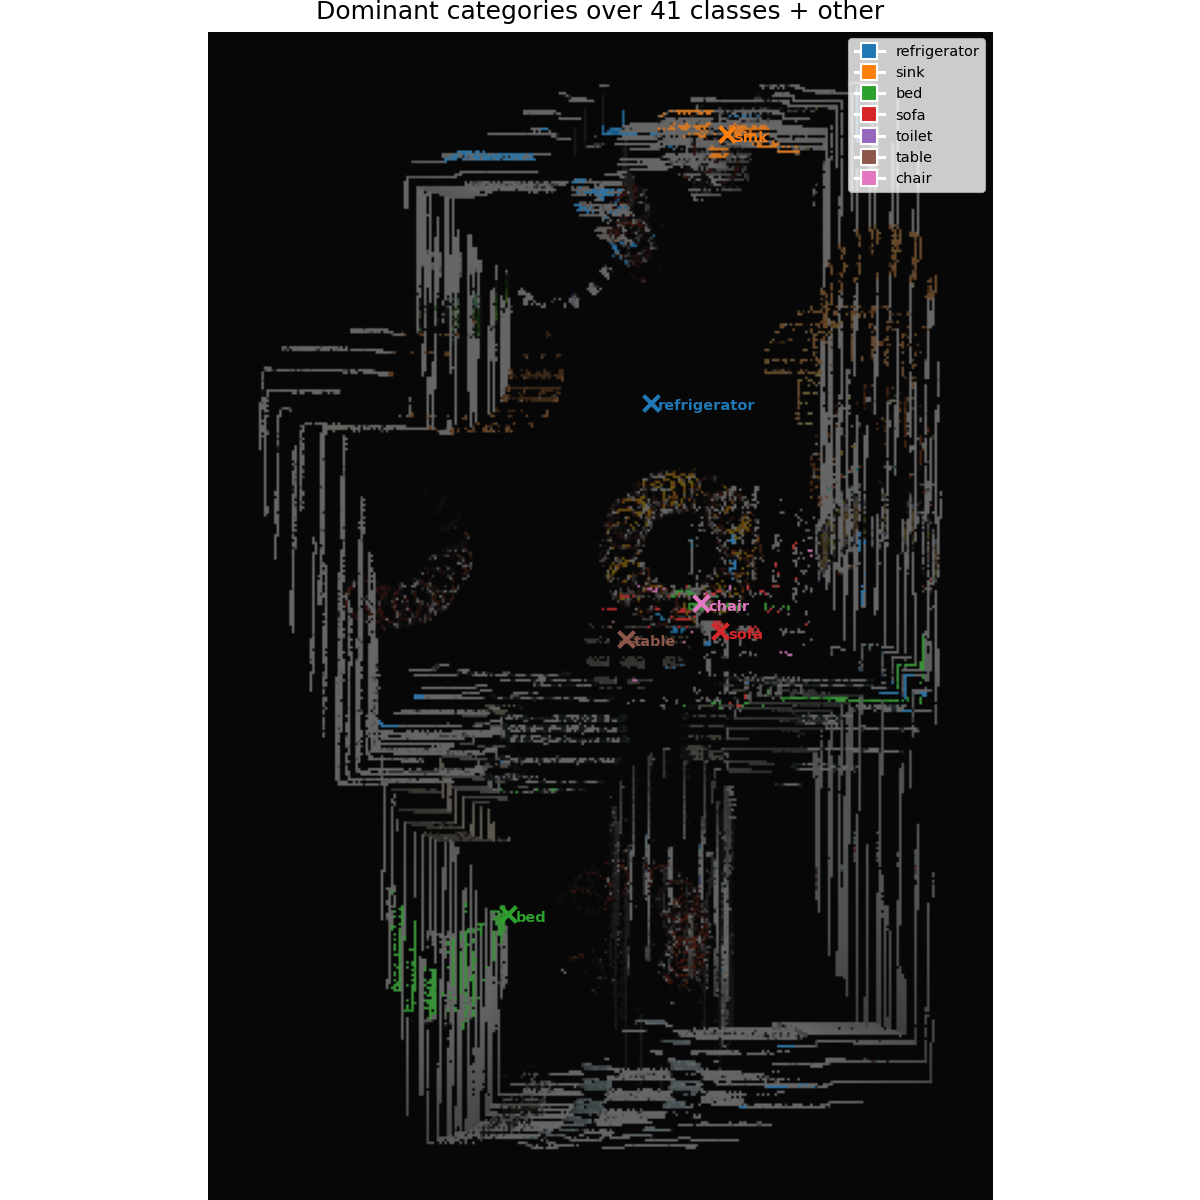
\includegraphics[width=0.48\linewidth]{figs/vlmap_index_small_house.png}
\hfill
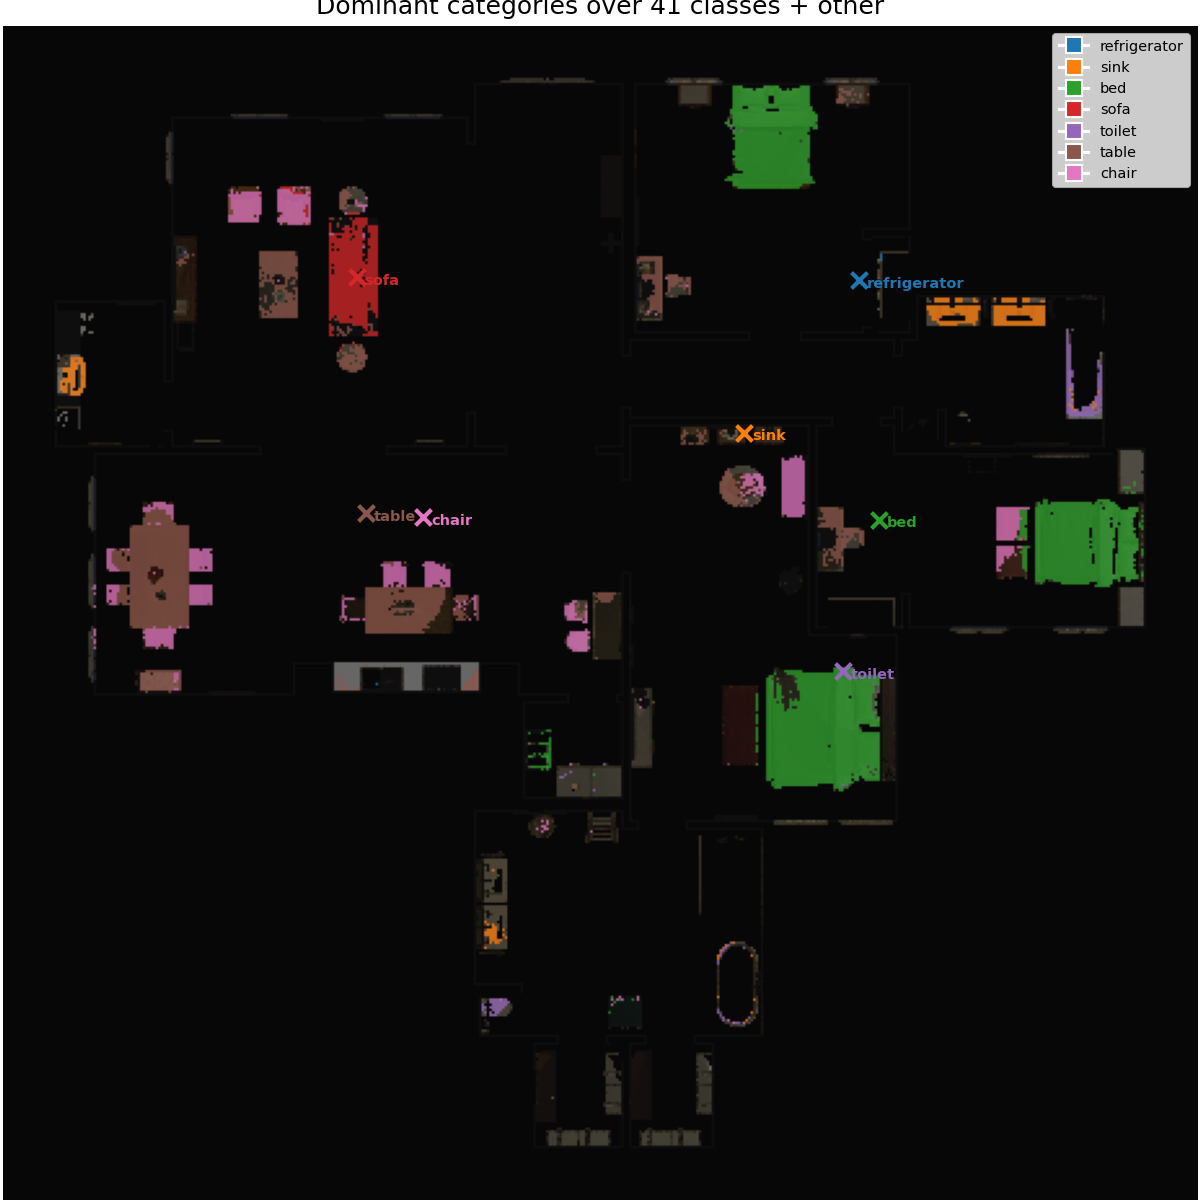
\includegraphics[width=0.48\linewidth]{figs/vlmap_index_hssd_102344280_0.png}
\caption{Validación sin interfaz gráfica del índice multiclase para el mapa capturado desde
ROS/Gazebo (izquierda) y para un mapa HSSD de referencia (derecha).}
\end{figure}

\paragraph{Pendiente para la siguiente iteración.}
\begin{itemize}
  \item Validar la captura real contra \texttt{small\_house} y
        \texttt{wrs} (verificación visual de que las nubes de puntos
        cubren las habitaciones esperadas).
  \item Ajustar \texttt{base2cam\_tf} y \texttt{base\_transform} en la
        configuración de VLMaps para la convención de la HSR (la actual
        está calibrada para Habitat).
  \item Conectar los candidatos publicados a \texttt{move\_base} para
        cerrar el bucle de navegación dentro de Gazebo.
\end{itemize}

\end{document}
